\chapter{Einführung}

Zum Einstieg werden wichtige Begriffe der Programmierung definiert:

\begin{description}
	\item[Programmiersprache:] formal konstruierte Sprache, entworfen um Befehle an Maschinen (speziell Computer) zu übermitteln. Gemeinsame Sprache zwischen Mensch und Maschine.
	\item[Syntax:] Gibt das Muster (die formale Struktur) vor, nach dem Programme einer Sprache aufgebaut sind (\textit{Zusammenfügungsregeln}).
	\item[Semantik:] Definiert die \textit{Bedeutung} von Programmen (Anweisungen, Operatoren, usw.) (\textit{Interpretationsregeln}).
	\item[Programmierparadigma:] fundamentaler Programmierstil, eine bestimmt Art die Struktur und Elemente von Programmen aufzubauen. Man kann mit allen Programmiersprachen die gleichen Probleme lösen (sind alle Turing-Vollständig), aber nicht gleich elegant.
	\item[Algorithmus:] Verfahren zur Lösung von einem Problem oder einer Klasse von Problemen.
\end{description}

Abbildung \ref{fig:programmierparadigmen} zeigt einen Überblick über die verschiedenen Programmierparadigmen. Fundamental ist die Unterscheidung in imperative und deklarative Programmiersprachen. Es gibt auch noch weitere Paradigmen (z.B. Aspekt-orientiert, Ereignis-orientiert), aber diese sind keine eigenen Programmiersprachen sondern in andere integriert. Die Unterscheidung ist nicht messerscharf (Deklarative Sprachen haben meist auch imperative Eigenschaften). Programmierparadigmen sind eher komplementär (d.h.
sich ergänzend) als sich gegenseitig ausschliessend.

\begin{figure}
\centering
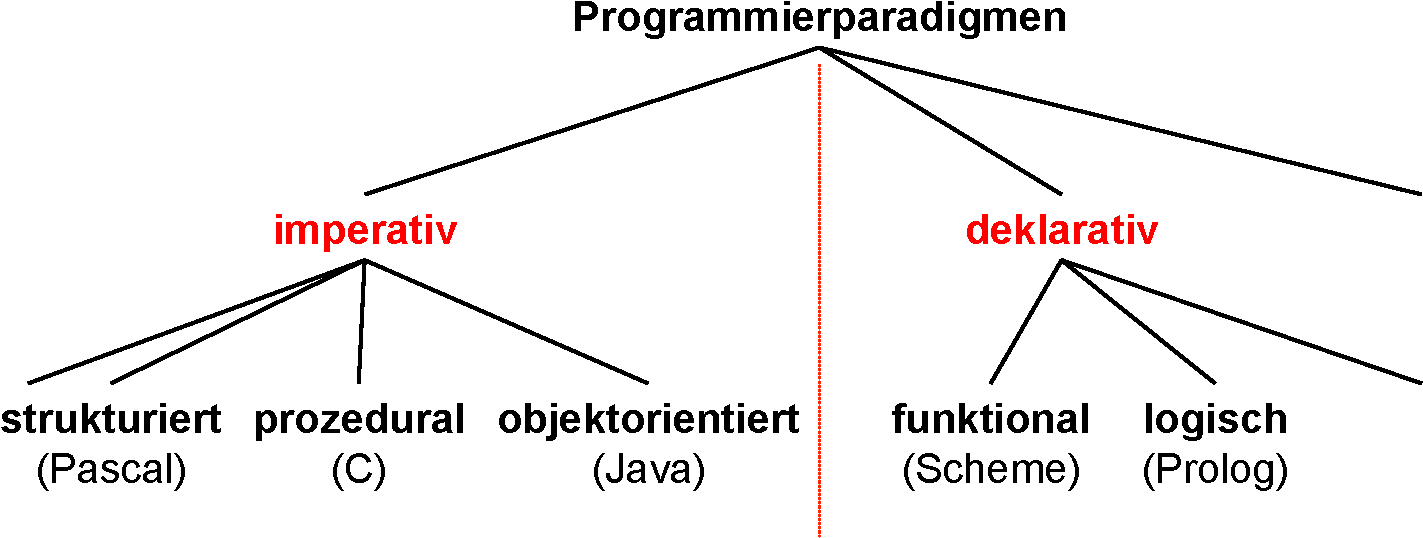
\includegraphics[width=0.7\linewidth]{fig/programmierparadigmen}
\caption{Überblick Programmierparadigmen}
\label{fig:programmierparadigmen}
\end{figure}

\section{Imperative Programmiersprachen}

Imperative Programmiersprachen beschreiben \textbf{wie} ein Problem gelöst werden kann (Tu das, tu das usw. und das Problem ist gelöst). Problem-Lösungs-Algorithmus wird schrittweise durch Befehle angegeben: Der Quellcode gibt an, was der Computer in welcher Reihenfolge tun soll. Zur Steuerung der Befehlsausführung stehen Kontrollstrukturen (Sequenz, Schleife [Iteration], Verzweigung [Selektion]) zur Verfügung. Imperatives Programmierparadigma ist eng angelehnt an die Ausführung von Maschinen-Code (Assembler) auf Computern, die nach der Von-Neumann-Architektur implementiert sind.

\subsection{Strukturierte Programmierung}

Verlangt Beschränkung auf drei \textbf{Kontrollstrukturen}:
\begin{enumerate}
	\item Sequenzen (Hintereinander auszuführende Programmanweisungen)
	\item Auswahl (Verzweigung: Bedingung)
	\item Wiederholung (Schleifen)
\end{enumerate}
Deshalb darf die \texttt{goto}-Anweisung nicht verwendet werden (sonst wird Dijkstra wütend!). Typische Sprachen: C, Fortran, Pascal.

\subsection{Prozedurale Programmierung}

Bietet Unterteilung von Programmen in Teilprogramme (Prozedur, Funktion usw.). Dadurch können Code-Duplikationen verhindert werden. Ist oft \textit{Gegenstück} zu OOP. Typische Sprachen: C, Fortran, Pascal.

\subsection{Objektorientierte Programmierung}

Laufende Programme bestehen aus einzelnen Objekte, welche miteinander interagieren. Objekte sind typischerweise Instanzen von Klassen (Geht auch anders, z.B. mit Prototypen in JavaScript). Klassen definieren Zustand (Variablen) und Verhalten (Methoden). Typische Sprachen: Smalltalk, Objective C, C++, Java, C\#.

\section{Deklarativen Programmiersprachen}

Deklarative Programmiersprachen beschreiben \textbf{was} das Problem ist (ohne Kontrollfluss). Das zu lösende Problem wird beschrieben, der Lösungsweg wird dann automatisch ermittelt: Das Programm enthält genügend Information, sodass das Problem gelöst werden kann.

\subsection{Logische Programmierung}

Programm besteht aus Fakten und Regeln, aus welchen auf Anfrage automatisch versucht wird, eine Lösungsaussage herzuleiten (Lösungsweg wird nicht angegeben). Basiert auf mathematischer Logik (Das war ja logisch...). Bekannteste Sprache: Prolog.

\subsection{Funktionale Programmierung}

Programme bestehen ausschliesslich aus Definitionen von Funktionen mit Parametern und Rückgabewerten. Der Rückgabewert hängt ausschliesslich von den Parametern ab. Es gibt keinen Zustand und keine veränderbaren Daten. Basiert auf Lambda-Kalkül. Bekannteste Sprachen: Clojure, Erlang, Haskell, Lisp, ML, Scheme.